\documentclass[12pt]{report}

\usepackage{commands}


\begin{document}

\large

\begin{center}
 Math 568 Homework 4\\
 Due February 3\\
 By Marvyn Bailly\\
\end{center}

\normalsize

\hrule

%---------------%
%---Problem 1---%
%---------------%

%--status--$

\begin{problem}
    Consider the weakly nonlinear oscillator:
    \[ 
        \ddn{2}{y}{t} + y + \eps y^5 = 0,
    \]
    with $y(0) = 0$ and $y'(0) = A > 0$ and with $0 < \eps \ll 1.$
    \begin{enumerate}
        \item [(a)]
        Use a regular perturbation expansion and calculate the first two terms. 
        

        \item [(b)]
        Determine at what time the approximation of part (a) fails to hold.
        

        \item [(c)]
        Use a Poincare-Lindstedt expansion and determine the first two terms and frequency corrections.
        
        
        \item [(d)]
        For $\eps = 0.1$, plot the numerical solution (from MATLAB), the regular expansion solution, and
        the Poincare-Lindstedt solution for $0 \leq t \leq 20$.
        


    \end{enumerate}
\end{problem}

\begin{solution}

    \noindent
    Consider the weakly nonlinear oscillator:
    \begin{equation} \label{oscillator}
        \ddn{2}{y}{t} + y + \eps y^5 = 0,
    \end{equation} 
    with $y(0) = 0$ and $y'(0) = A > 0$ and with $0 < \eps \ll 1.$
    \begin{enumerate}
        \item [(a)]
        First we wish to compute the first two terms of the regular perturbation expansion. First let
        \[ 
            y(t) = y_0 + \eps y_1(t) + \eps^2 y_2(t) + \cdots.
        \] 
        Substituting this into Eq. (1) yields
        \[ 
            (y''_0 + \eps y''_1 + \cdots) + (y_0 + \eps y_1 + \cdots) + \eps(y_0 + \eps y_1 + \cdots)^5 = 0.
        \] 
        Next we can collect the terms in powers of $\eps$ which gives
        \begin{align*}
            &\O(1):      &&y''_0 + y_0 = 0,  &&&y_0(0) = 0, y'_0(0) = A,\\
            &\O(\eps):   &&y''_1 + y_1 + y_0^5 = 0, &&&y_1(0) = 0, y'_1(0) = 0,\\
            &\O(\eps^2): &&y''_2 + y_2 + 5y_0^4y_1 = 0,  &&&y_2(0) = 0, y_2'(0) = 0.
        \end{align*}  
        The leading order problem
        \[ 
            y''_0 + y_0 = 0,
        \]
        with boundary conditions $y_0(0) = 0$ and $y_0'(0) = A$ has the general solution 
        \[ 
            y_0(t) = c_1 \cos(t) + c_2\sin(t),
        \]
        and applying the first boundary condition gives $c_1 =0$ which yields the solution 
        \[ 
            y_0(t) = c_2\sin(t).
        \]
        Enforcing the second boundary conditions gives $c_2 = A$ and thus the final solution is 
        \[ 
            y_0(t) = A\sin(t),
        \]
        which is the first term in the regular perturbation expansion. Substituting this solution into the $\O(\eps)$ equation yields
        \[ 
            y''_1 + y_1 = -A^5\sin^5(t),
        \]
        with boundary conditions $y_1(0) = 0$ and $y_1'(0)=0$ which is a second order inhomogeneous differential equation. To solve this differential equation, we need to use the method of variation parameters. First let's solve the homogeneous problem
        \[ 
            y''_1 + y_1 = 0,
        \]
        which has the general solution 
        \[ 
            y_1(t) = c_1\cos(t) + c_2\sin(t).
        \]
        Next, we can find the particular solution by computing
        \[ 
            y_p(t) = -\bar{y}_1(t)\int\frac{\bar{y}_2(t)f(t)}{W(\bar{y}_1(t),\bar{y}_2(t))}dt + \bar{y}_2(t) \int \frac{\bar{y}_1(t)f(t)}{W(\bar{y}_1(t),\bar{y}_2(t))}dt,
        \]
        where $f(t) = -A^5\sin^5(t)$, $\bar{y}_1(t) = \cos(t)$ and $\bar{y}_2(t) = \sin(t)$. This yields
        \[ 
            y_p(t) = \frac{1}{384} A^5 (-80 \sin (t)-15 \sin (3 t)+\sin (5 t)+120 t \cos (t)),
        \]
        and thus the general solution is given by
        \[ 
            y_1 = c_1\cos(t) + c_2\sin(t) + \frac{1}{384} A^5 (-80 \sin (t)-15 \sin (3 t)+\sin (5 t)+120 t \cos (t)),
        \]
        and enforcing the boundary conditions gives
        \[ 
            y_1 = \frac{1}{384} A^5 (-80 \sin (t)-15 \sin (3 t)+\sin (5 t)+120 t \cos (t)).
        \]
        Thus we have found the first two terms of the regular perturbation expansion to be
        \[ 
            y(t) = A\sin(t) + \eps\paren{\frac{1}{384} A^5 (-80 \sin (t)-15 \sin (3 t)+\sin (5 t)+120 t \cos (t))} + \O(\eps^2).
        \] 

        \item [(b)]
        In the second term of the regular perturbation expansion we have a secular growth term that shows the perturbation is the same size as the leading order solution at $t ~ \O(1/\eps)$. Thus for $t$ values greater than $\O(1/\eps)$, the solution blows up to infinity.
        
        \def\w{\omega}

        \item [(c)]
        Now we wish to use the Poincare-Lindstedt expansion to remove the secular term. We begin by letting
        \begin{align*}
            \tau &= \w(\eps)t ~~\text{where}~~\w(\eps) = \w_0 + \eps\w_1 + \eps^2\w_2 + \dots,\\
            y &= y_0 + \eps y_1 + \eps^2y_2 + \dots.
        \end{align*} 
        Note that by the chain rule $y_{tt} = \w^2 y_{\tau \tau}$. Plugging these into the Eq. (1) and collecting terms yields
        \begin{align*}
            &O(1): &&\w_0 y_{0_{\tau \tau}} + y_0 = 0, &&&y_0(0) = 0, w_0y_{0_\tau}(0)=A,\\
            &O(\eps): && y_{1_{\tau \tau}} + y_1 = -2\w_1y_{0_{\tau \tau}} -  y_0^5, &&&y_1(0) = 0, \w_1y_{0_\tau} + \w_0 y_{1_\tau} = 0.\\
        \end{align*}
        Let's first solve the leading order term
        \[ 
            \w_0 y_{0_{\tau \tau}} + y_0 = 0.
        \]
        Enforcing the Fredholm-Alternative theorem
        \[ 
            \abrac{0,\sin\tau}=0,
        \]
        shows that the solvability of the leading order always satisfied and thus independent of $\w_0$. Thus let's let $\w_0 = 1$. The general solution to the leading order term is given by
        \[ 
            c_1\cos(\tau) + c_2\sin(\tau) = 0,
        \] 
        and applying the boundary conditions $y_0(0) = 0, y_{0_\tau}(0)=A$ gives the leading order term to be
        \[ 
            y_0 = A\sin(\tau).
        \]
        Plugging the found values into the $\O(\eps)$ term gives 
        \[ 
            y_{1_{\tau \tau}} + y_1 = 2\w_1A\sin(\tau) - A^5 \sin^5(\tau), ~~~ y_1(0) = 0,  y_{1_\tau} = -\w_1A.
        \]
        Enforcing the Fredholm-Alternative theorem, applying the trig identify $\sin^5(\tau) = \frac{10\sin(\tau) - 5\sin(3\tau) + \sin(5\tau)}{16}$, and noting that $\sin(\tau)$ is orthogonal to $\sin(3\tau)$ and $\sin(5\tau)$ gives 
        \begin{align*}
            &\abrac{2\w_1A\sin(\tau) - A^5 \sin^5(\tau),\sin(\tau)} = 0\\
            &\iff \abrac{2\w_1\sin(\tau) - A^4 \paren{\frac{10\sin(\tau) - 5\sin(3\tau) + \sin(5\tau)}{16}},\sin(\tau)} = 0\\
            &\iff \abrac{2\w_1\sin(\tau) - \frac{10A^4}{16}\sin(\tau),\sin(\tau)} = 0\\
            &\iff \paren{2\w_1 - \frac{10A^4}{16}}\abrac{\sin(\tau), \sin(\tau)} = 0.
        \end{align*} 
        As $\abrac{\sin(\tau), \sin(\tau)} \neq 0$ we find that
        \[ 
            \w_1 = \frac{5}{16}A^4.
        \]
        Plugging this back into the $\O(\eps)$ term gives
        \[ 
            y_{1_{\tau \tau}} + y_1 = \frac{5}{8}A^4\sin(\tau) - A^5 \sin^5(\tau), ~~~ y_1(0) = 0,  y_{1_\tau} = - \frac{5}{16}A^5.
        \]
        To solve the ODE, we use variation of parameters to get the homogeneous solution
        \[ 
            \hat{y}_1 = B\sin(\tau) + C\cos(\tau),
        \]
        and the particular solution 
        \[ 
            y_{1_p} = \frac{1}{384} A^5 (-80 \sin (\tau)-15 \sin (3 \tau)+\sin (5 \tau)).
        \]
        Adding the two solution together and applying the boundary conditions $y_1(0) = 0,  y_{1_\tau} = - \frac{5}{16}A^5$ gives $\O(\eps)$ solution to be
        \[ 
            y_1 = \frac{1}{384} A^5 (-80 \sin (\tau)-15 \sin (3 \tau)+\sin (5 \tau)).
        \]
        Therefore we have found the first two terms of the Poincare-Lindstedt expansion to be
        \[ 
            y = A\sin((1 + \eps\frac{ 5}{16}A^4)t) + \frac{\eps}{384} A^5 (-80 \sin ((1 + \eps\frac{ 5}{16}A^4)t)-15 \sin (3 (1 + \eps\frac{ 5}{16}A^4)t)+\sin (5 (1 + \eps\frac{ 5}{16}A^4)t)) + \cdots,
        \] 
        and the first two frequency corrections
        \[ 
            \w_0 = 1 ~~~ \text{and}~~~ \w_1 = \frac{5}{16}A^4.
        \]


        \item [(d)]
        Using Mathematica to plot the numerical solution (using \verb+NDSolve+), the regular expansion solution, and
        the Poincare-Lindstedt solution for $0 \leq t \leq 20$ with $\eps = 0.1$ gives the following plots:
        \begin{figure}[H]
            \center
            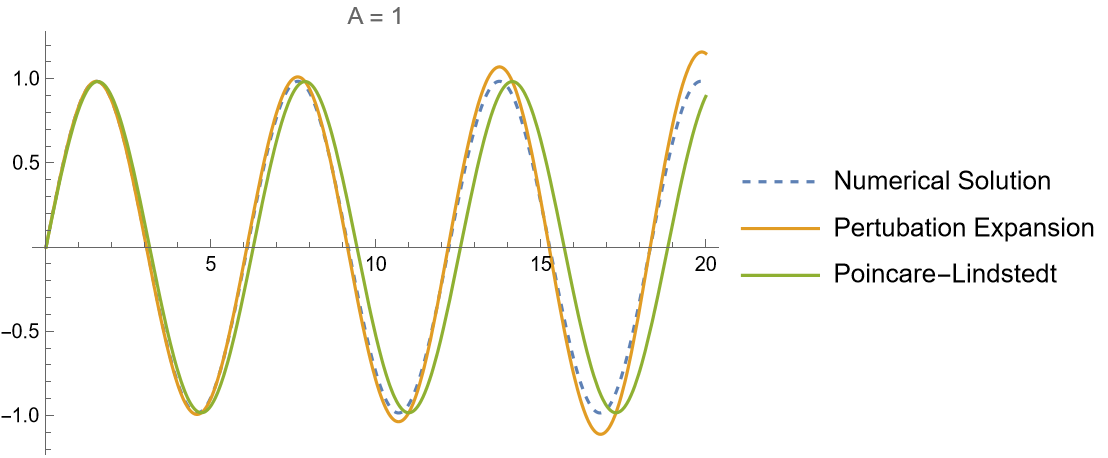
\includegraphics[width=.8\textwidth]{plots/1d.png}
            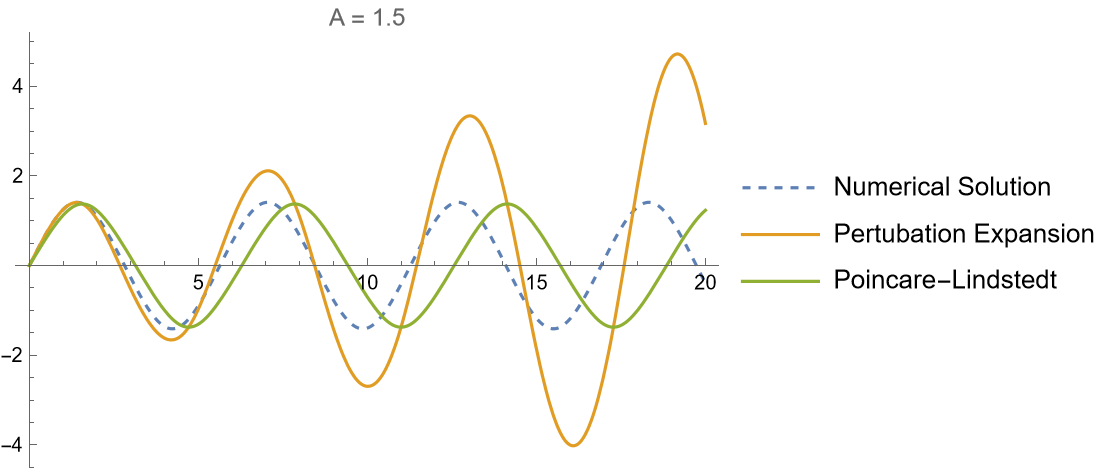
\includegraphics[width=.8\textwidth]{plots/1d1.png}
            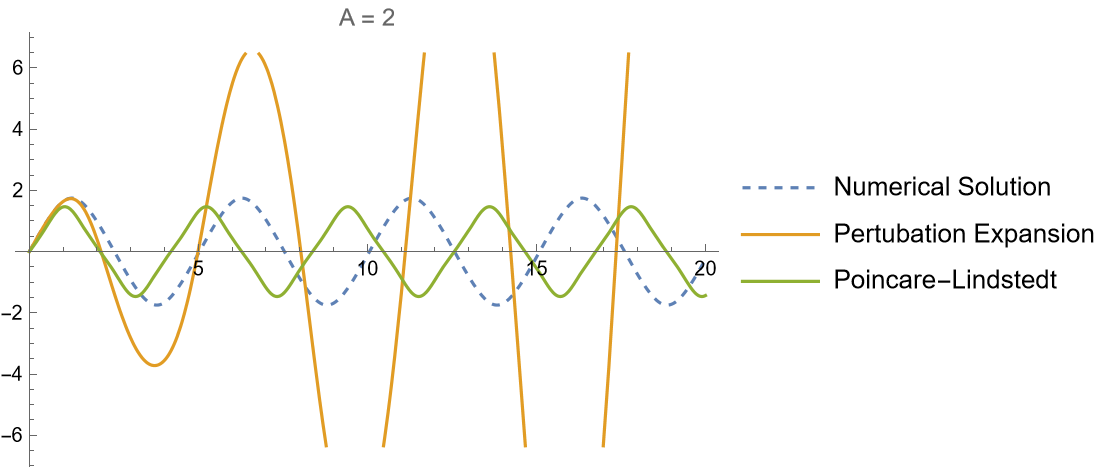
\includegraphics[width=.8\textwidth]{plots/1d2.png}
        \end{figure}
        We see that the perturbation expansion is accurate until $\O(1/\eps)$ and then the secular term causes the solution to blow up. On the other hand, the Poincare-Lindstedt solution does not have a secular term and does not blow up but differs in frequency to the numerical solution. 

    \end{enumerate}
\end{solution}

%----------------------------------------------------------------------------------------------------%
%\vskip 20pt
\newpage

%---------------%
%---Problem 2---%
%---------------%

%--status--$

\begin{problem}
    Consider Rayleigh's equation
    \[ 
        \ddn{2}{y}{t} + y + \eps \left[ - \dd{y}{t} + \frac{1}{3}\paren{\dd{y}{t}}^3\right] = 0,
    \]
    which has only one periodic solution called a "limit cycle" ($0 < \eps \ll 1$). Given
    \[ 
        y(0) = 0,
    \]
    and
    \[ 
        \dd{y(0)}{t} = A.
    \]
    \begin{enumerate}
        \item [(a)]
        Use a multiple scale expansion to calculate the leading order behavior.


        \item [(b)]
        Use a Poincare-Lindsted expansion and an expansion of $A = A_0 + \eps A_1 + \cdots$ to calculate the
        leading-order solution and the first non-trivial frequency shift for the limit cycle.


        \item [(c)]
        For $\eps = 0.01, 0.1, 0.2,$ and $0.3$, plot the numerical solution and the multiple scale expansion for
        $0 \leq t \leq 40$ and for various values of $A$ for your multiple scale solution. Also plot the limit cycle
        solution calculated from part (b).

        \item [(d)]
        Calculate the error 
        \[ 
            E(t) = |y_{\text{numerical}}(t) - y_{\text{approximation}}(t)|,
        \]
        as a function of time ($0 \leq t \leq 40$) using $\eps = 0.01, 0.1, 0.2,$ and $0.3$. 

    \end{enumerate}
\end{problem}

\begin{solution}
    
    \noindent
    \begin{enumerate}
        \def\w{\omega}



        \item [(a)]
        Consider Rayleigh's equation
        \[ 
            y'' + y + \eps \paren{-y' + \frac{1}{3}y'^3 } = 0
        \]
        with the initial conditions
        \[ 
            y(0) = 0 ~~~ \text{and} ~~~ y'(0) = \alpha. 
        \]
        First we wish to use a multiple scale expansion to calculate the leading order behavior. The scaling takes the form
        \[ 
            y = y_0(x,t,\tau) + \eps y_1(x,t,\tau) + \dots, 
        \]
        where $\tau = \eps t$ is the slow variable dependence. Note that the chain rule gives 
        \begin{align*}
            y_{t} &= y_{t} + \eps y_{\tau},\\
            y_{tt} &= y_{tt} + 2\eps y_{t\tau} + \eps^2y_{\tau \tau}.
        \end{align*}
        Plugging these into Rayleigh's equation gives
        \[ 
            (y_{tt} + 2\eps y_{t\tau} + \eps^2y_{\tau \tau}) + y + \eps\paren{-( y_{t} + \eps y_{\tau}) + \frac{1}{3}( y_{t} + \eps y_{\tau})^3} = 0,
        \]
        with the initial conditions $y(0,0) = 0$ and $y'(0,0) = \alpha$. Next collect terms to get
        \begin{align*}
            &\O(1): &&y_{0_{\tau \tau}} + y_0 = 0 &&&y_0(0,0) = 0,y_{0_t}(0,0) = \alpha,\\
            &\O(\eps): &&y_{1_{tt}} + y_1 = - 2y_{0_{t\tau}} + y_{0_t} - \frac{1}{3}y_{0_t}^3 &&&y_1(0,0)=0, y_{1_t}(0,0) = -y_{0_\tau}(0,0).
        \end{align*}  
        The leading order solution produces the general solution
        \[ 
            y_0(t,\tau) = A(\tau)\cos(t) + B(\tau)\sin(t)
        \]
        where $A(0) = 0$ and $B(0) = \alpha$. Plugging the leading order solution into the $\O(\eps)$ equation gives
        \begin{align*}
            y_{1_{tt}} + y_1 = -2(-\sin(t)A'(\tau) + \cos(t)B'(\tau)) &+ B(\tau)\cos(t) - A(\tau)\sin(t)\\ 
            &- \frac{1}{3} \paren{B(\tau)\cos(t)- A(\tau)\sin(t)}^3.
        \end{align*} 
        Using trig identities $\sin^3(t) = \frac{3}{4}\sin(t) - \frac{3}{4}\sin(3t)$ and $\cos^3(t) = \frac{3}{4}\cos(t) + \frac{1}{4}\cos(3t)$, we can rewrite the right hand side as
        \begin{align*}
            y_{1_{tt}} + y_1 = &\paren{2A' - A - \frac{1}{3}\paren{-\frac{3}{4}AB^2 - \frac{3}{4}A^3}}\sin(t)-\frac{1}{3}\paren{\frac{1}{4}A^3 - \frac{3}{4}AB^2}\sin(3t)\\
            &+\paren{B-2B'-\frac{1}{3}\paren{\frac{3}{4}B^3-\frac{1}{4}A^2B}}\cos(t)-\frac{1}{3}\paren{\frac{1}{4}B^3 - \frac{3}{4}A^2B}\cos(3t).\\
        \end{align*}
        Now we wish to eliminate the terms that cause secular growth which gives us the following system of ODEs
        \begin{align}
            2A' - A - \frac{1}{3}\paren{-\frac{3}{4}AB^2 - \frac{3}{4}A^3} &= 0\\
            B-2B'-\frac{1}{3}\paren{\frac{3}{4}B^3-\frac{1}{4}A^2B} &= 0.
        \end{align}
        Multiplying the Eq. (2) by $A$ and Eq.(3) by $B$ and adding them together yields
        \[ 
            \rho_\tau + \frac{1}{4}\rho^2 - \rho = 0,
        \]  
        where $\rho = A^2 + B^2$. Noticing that this is Bernoulli equation of the form
        \[ 
            \rho^{-2}\rho - \rho^{-1} = -\frac{1}{4},
        \]
        gives that
        \[ 
            \rho = \frac{4}{1 + c e^{-\tau}},
        \]
        where $c$ is an integration constant. Applying the initial conditions $\rho(0) = A^2(0) + B^2(0) = \alpha$ gives 
        \[ 
            c = \frac{4 - \alpha^2}{\alpha^2},
        \]
        and thus
        \[ 
            \rho = \frac{4\alpha^2}{\alpha^2 + (4-\alpha^2)e^{-\tau}} = A^2 + B^2.
        \]
        Solving for $B^2$ and substituting into Eq. (2) gives
        \[ 
            2A' - A - \frac{1}{3}\paren{-\frac{3}{4}A(\rho - A^2) - \frac{3}{4}A^3} = 0
        \]
        and applying the boundary condition $A(0) = 0$ shows that $A(\tau) = 0$. Thus $B = \sqrt{\rho}$.  Therefore the leading order behavior of the multiple scale expansion is
        \[ 
            y(t) = \paren{\sqrt{\frac{4\alpha^2}{\alpha^2 + (4-\alpha^2)e^{-\eps t}}}}\sin(t) + \O(\eps).
        \] 

        \item [(b)]
        Next we wish to apply a Poincare-Lindstedt expansion 
        \[ 
            \tau = \w t = (\w_0 + \eps\w_1 + \cdots)t,
        \]
        and the expansion
        \[ 
            \alpha = \alpha_0 + \eps\alpha_1 + \cdots.
        \]
        Plugging these expansion into Rayleigh's equation yields
        \[ 
            \w^2 y_{\tau \tau} + y + \eps\paren{-\w y_\tau + \frac{1}{3}\w^3 y_\tau^3} = 0,
        \]
        and collecting the leading order terms gives the following ODE with respect to the given initial conditions
        \[ 
            \w_0^2 y_{0_{\tau \tau}} + y_0 = 0, ~~~~ y_0(0) = 0, \w_0y_\tau(0)=\alpha_0.
        \]
        Noting that zero is in the null space and thus the Fredholm-Alternative theorem is satisfied regardless of the $\w_0$, pick $\w_0 = 1$. Finding the general solution and applying the initial conditions the leading order solution to be
        \[ 
            y_0 = \alpha_0 \sin(\tau). 
        \]
        To solve for $\alpha_0$, let's collect the $\O(\eps)$ terms
        \[ 
            \w_0^2y_{1_{\tau\tau}} + y_1 = -2\w_0\w_1y_{0_{\tau\tau}} + \w_0y_{0_\tau} - \frac{1}{3}w_0^3y_{0_\tau}^3, ~~~~ y_1(0)=0,y_{1_\tau}(0) + \w_1(y_{0_\tau}) = \alpha_1. 
        \] 
        Substituting $y_0$ and $\w_0$ into the equation we get
        \[ 
            y_{1_{\tau\tau}} + y_1 = 2\w_1\alpha_0\sin(\tau) + \alpha_0\cos(\tau)- \frac{1}{3}\alpha_0^3\cos(\tau)^3.
        \]
        Next we need to enforce the Fredholm-Alternative of the right hand side with both $\sin(\tau)$ and $\cos(\tau)$. Observe that
        \begin{align*}
            \abrac{2\w_1\alpha_0\sin(\tau) + \alpha_0\cos(\tau)- \frac{1}{3}\alpha_0^3\cos(\tau)^3,\sin(\tau)} &= 0\\
            2\w_1\alpha_0\abrac{\sin(\tau),\sin(\tau)} + 0 &= 0\\
            \implies 2\w_1\alpha_0 &= 0,
        \end{align*}
        and using $\cos^3(t) = \frac{3}{4}\cos(t) + \frac{1}{4}\cos(3t)$
        \begin{align*}
            \abrac{2\w_1\alpha_0\sin(\tau) + \alpha_0\cos(\tau)- \frac{1}{3}\alpha_0^3\cos(\tau)^3,\cos(\tau)} \\
            0 + \alpha_0 \abrac{\cos(\tau),\cos(\tau)}  - \frac{\alpha_0^3}{3}\abrac{\frac{3}{4}\cos(\tau)+\frac{1}{4}\cos(3\tau),\cos(\tau)} &= 0\\
            \paren{\alpha_0 + \frac{1}{4}\alpha_0^3}\abrac{\cos(\tau),\cos(\tau)} + 0 &= 0\\
            \implies \alpha_0 - \frac{1}{4}\alpha^3 &= 0.
        \end{align*}
        Thus we either have $\alpha_0 = 0$ or $\alpha_0 = 2$. Let's pick $\alpha_0 = 2$ and $\w_1 = 0$ giving us the following ODE subject to the initial conditions
        \[ 
            y_{1_{\tau\tau}} + y_1 = 2\cos(\tau)- \frac{8}{3}\cos(\tau)^3, ~~~y_1(0) = 0, y_{1_\tau}(0) = \alpha_1.
        \]
        Using variation of parameters and applying the initial condition gives the solution to be
        \[ 
            y_1 = \frac{1}{12} (12 \alpha_1 \sin (\tau)-\cos (\tau)+\cos (3 \tau)).
        \]
        To find the first non-trivial frequency shift, let's collect the $\O(\eps^2)$ terms
        \begin{align*}
            y_{2_{\tau \tau}} + y_2 &= y_{1_\tau} - y_{0_\tau}^2y_{1_\tau} - 2\w_2y_{0_{\tau\tau}}\\
            y_{2_{\tau \tau}} + y_2 &= \frac{1}{3} \cos ^2(\tau ) \left(12 \alpha _1 \cos (\tau ) +\sin (\tau )-3 \sin (3 \tau )\right)\\
            &+\frac{1}{12} \left(-12 \alpha _1 \cos (\tau )-\sin (\tau )+3 \sin (3 \tau )\right)-4 \omega _2 \sin (\tau ).
        \end{align*} 
        Using Mathematica to enforce the Fredholm-Alternative of the right hand side with both $\sin(\tau)$ and $\cos(\tau)$ and solve the resulting system of two ODEs gives that $\alpha_1 = 0$ and $\w_2 = - \frac{1}{16}.$ Therefore we have the leading order term to be 
        \[ 
            y = 2\sin((1 - \frac{\eps^2}{16})t) + \cdots
        \]
        with the first non-trivial frequency shift 
        \[ 
            \w_2 = - \frac{1}{16}
        \]
        \item [(c)]
        Using Mathematica we can create the following graphs for $\eps = 0.01, 0.1, 0.2,$ and $0.3$ for $A = 0.2, 2,$ and $20$ using the Poincare-Lindstedt expansion, multiscale expansion and Mathematica's numerical solution. We note that the limit cycle is at $A = 2$ so for $A$ values below $2$ we see the graph of the multiscale goes up to the solution and vice versa when $A$ is above $2$.  
        
        \begin{figure}[H]
            \center
            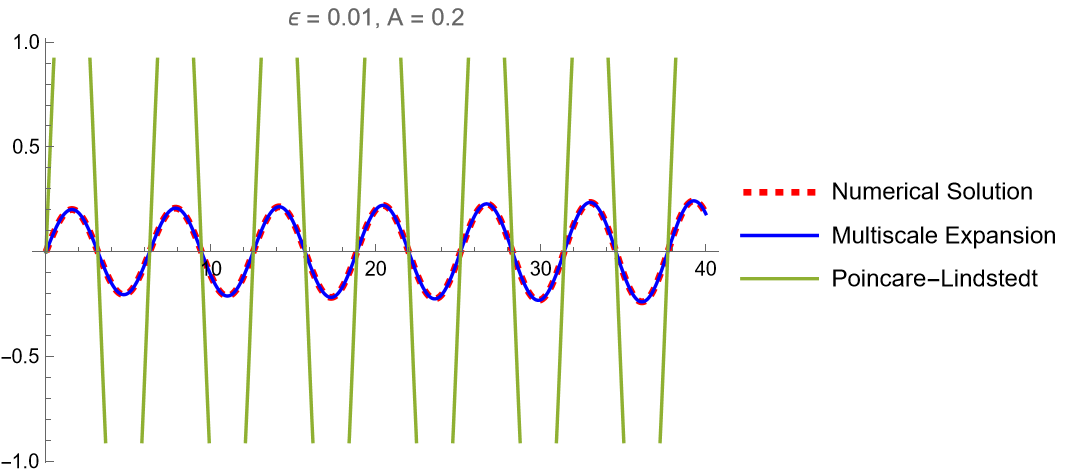
\includegraphics[width=.8\textwidth]{plots/2c1.png}
        \end{figure}
        \begin{figure}[H]
            \center
            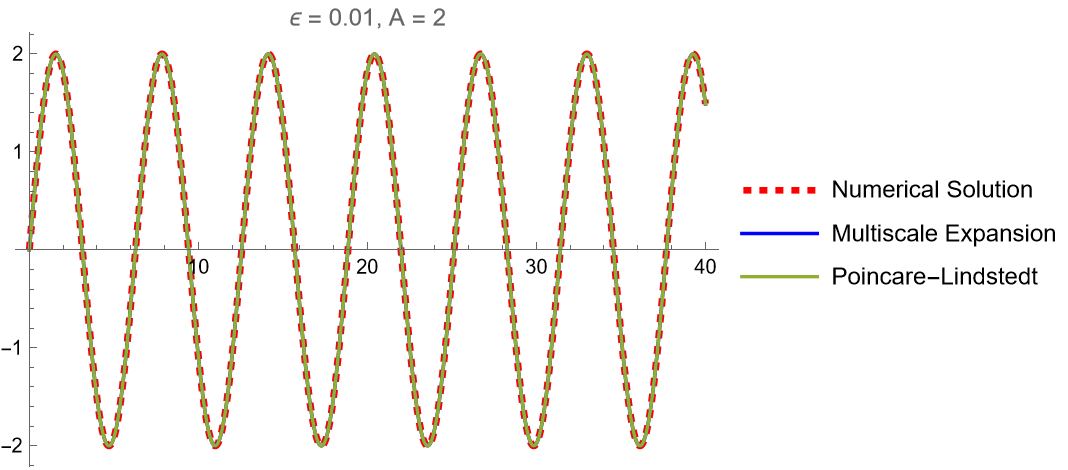
\includegraphics[width=.8\textwidth]{plots/2c2.png}
        \end{figure}
        \begin{figure}[H]
            \center
            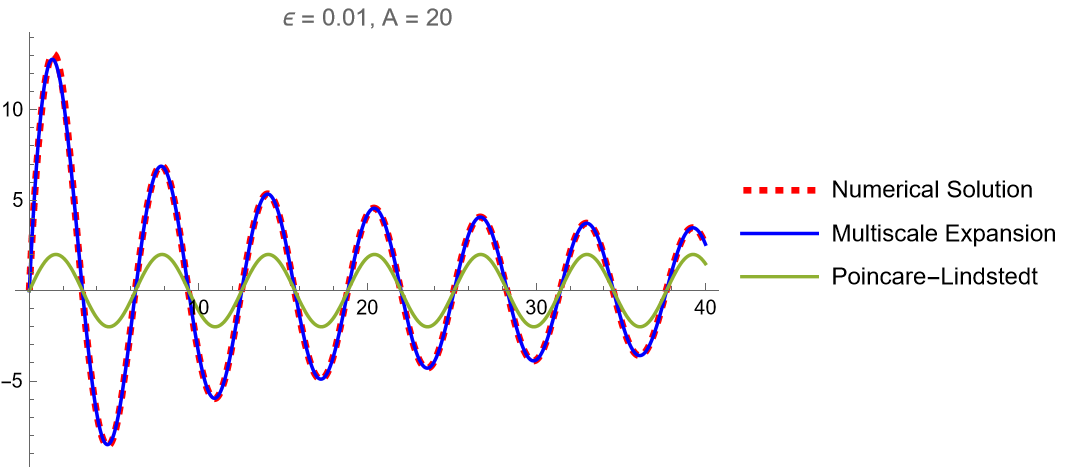
\includegraphics[width=.8\textwidth]{plots/2c3.png}
        \end{figure}
        \begin{figure}[H]
            \center
            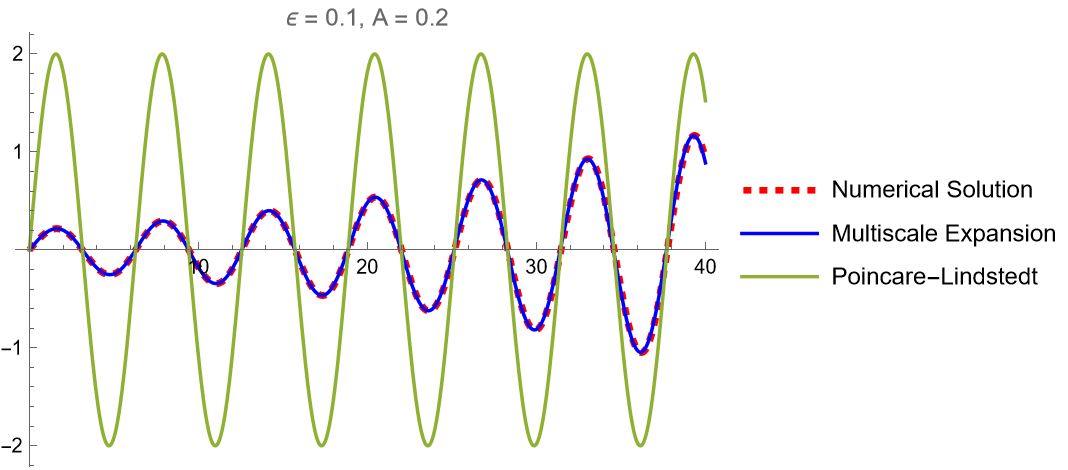
\includegraphics[width=.8\textwidth]{plots/2c4.png}
        \end{figure}
        \begin{figure}[H]
            \center
            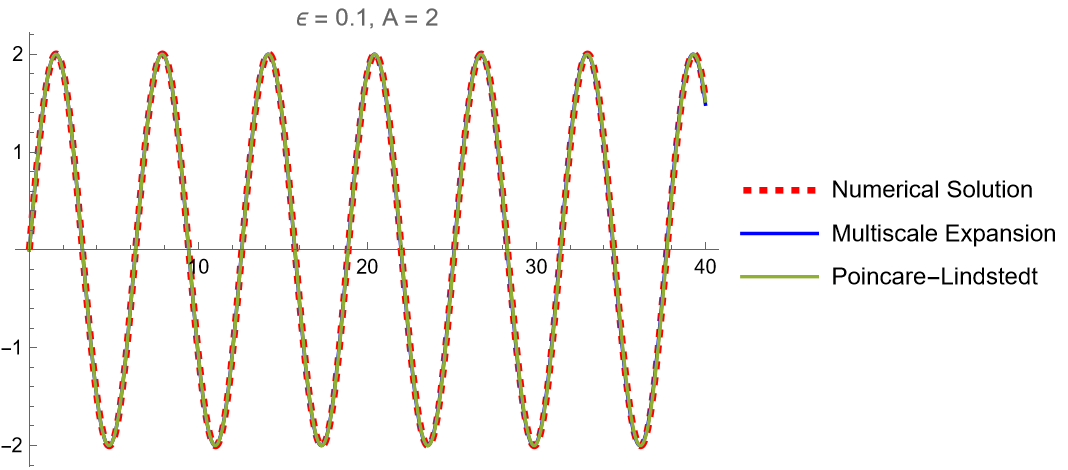
\includegraphics[width=.8\textwidth]{plots/2c5.png}
        \end{figure}
        \begin{figure}[H]
            \center
            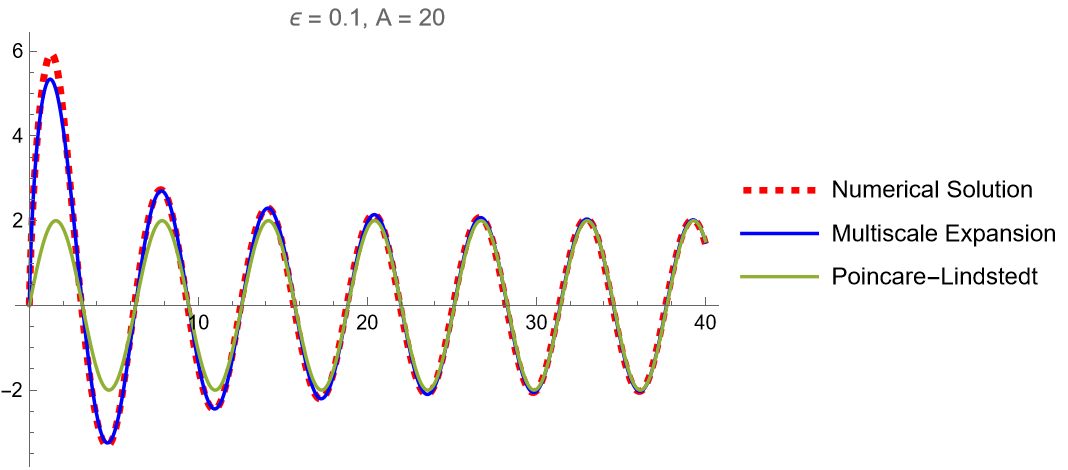
\includegraphics[width=.8\textwidth]{plots/2c6.png}
        \end{figure}
        \begin{figure}[H]
            \center
            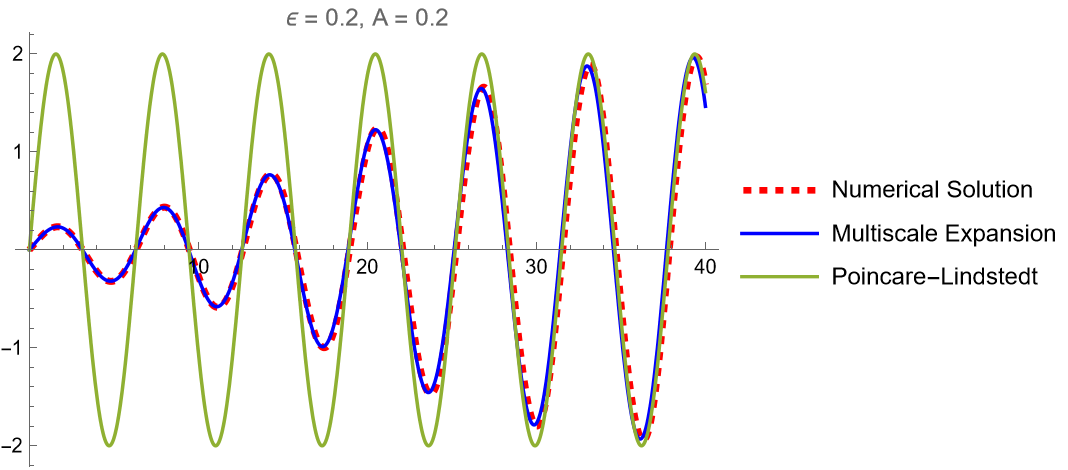
\includegraphics[width=.8\textwidth]{plots/2c7.png}
        \end{figure}
        \begin{figure}[H]
            \center
            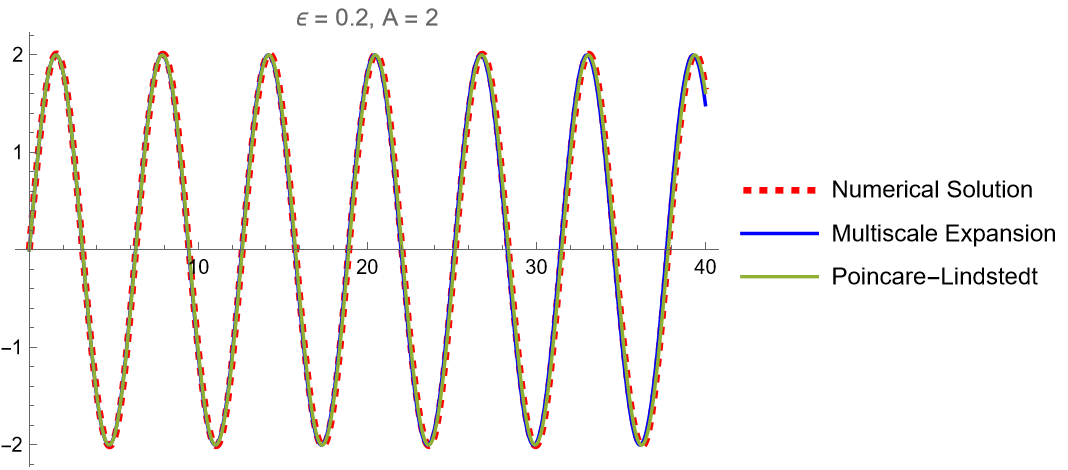
\includegraphics[width=.8\textwidth]{plots/2c8.png}
        \end{figure}
        \begin{figure}[H]
            \center
            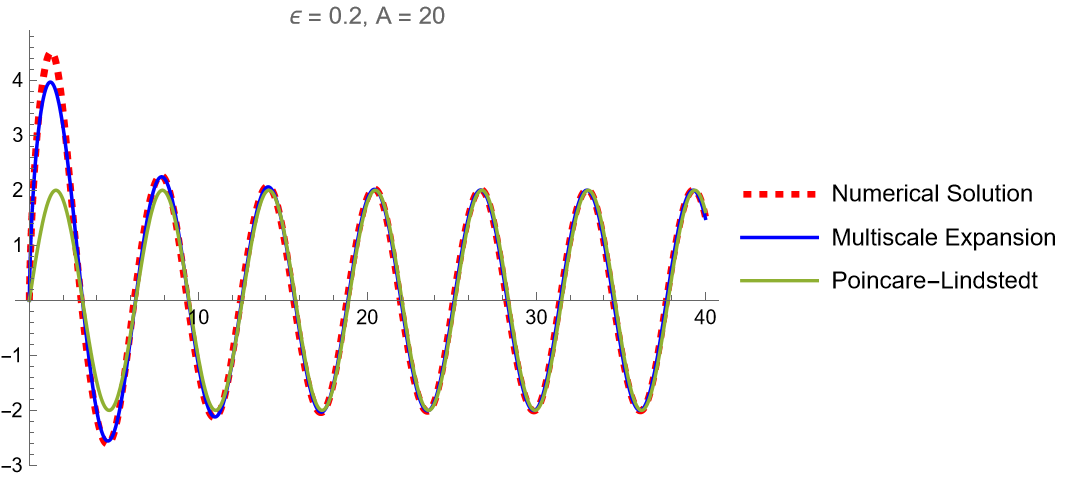
\includegraphics[width=.8\textwidth]{plots/2c9.png}
        \end{figure}
        \begin{figure}[H]
            \center
            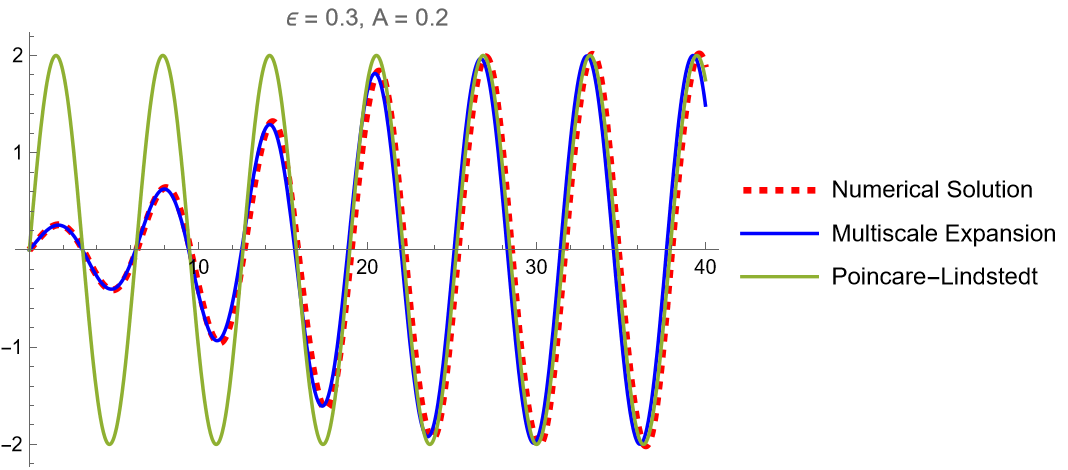
\includegraphics[width=.8\textwidth]{plots/2c10.png}
        \end{figure}
        \begin{figure}[H]
            \center
            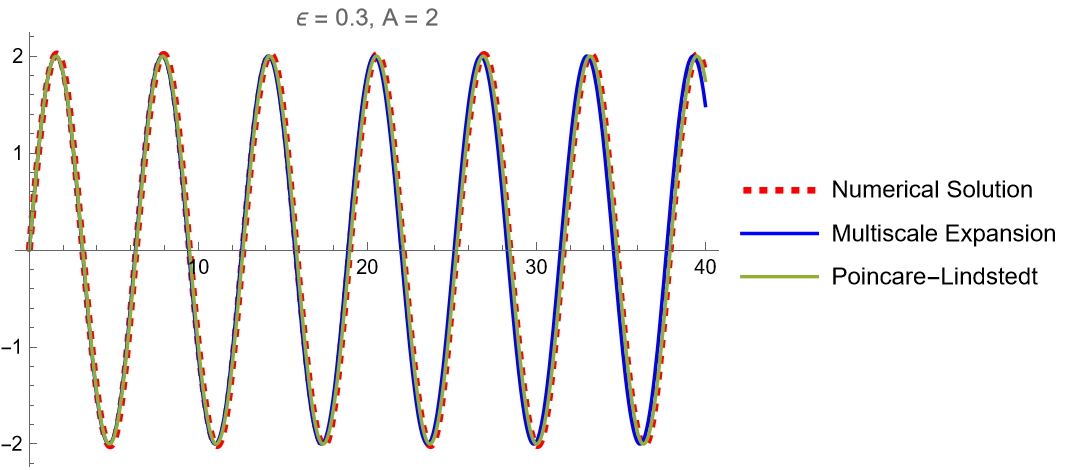
\includegraphics[width=.8\textwidth]{plots/2c11.png}
        \end{figure}
        \begin{figure}[H]
            \center
            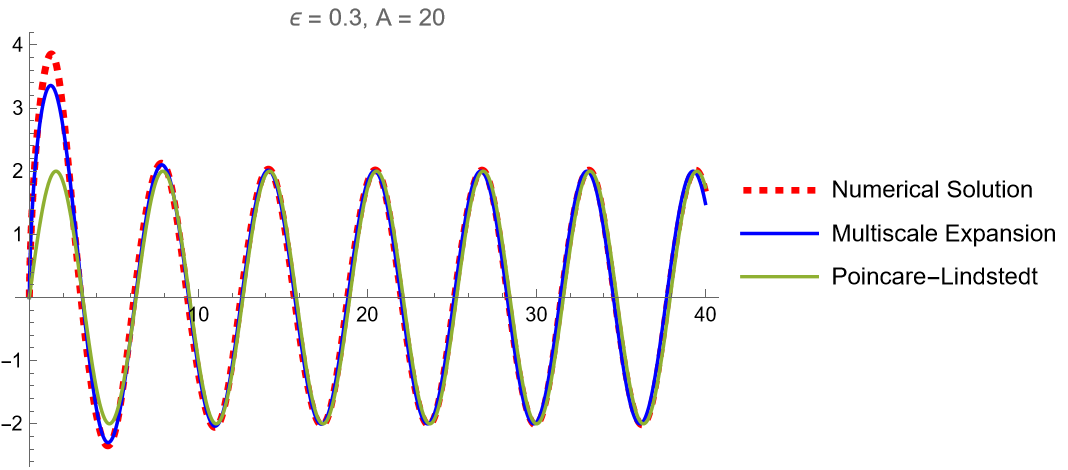
\includegraphics[width=.8\textwidth]{plots/2c12.png}
        \end{figure}
    
        \item [(d)]
        Next we wish to calculate the error of each approximation using
        \[ 
            E(t) = |y_{\text{numerical}}(t) - y_{\text{approximation}}(t)|,
        \]
        and Mathematica's numerical solution.
        \begin{figure}[H]
            \center
            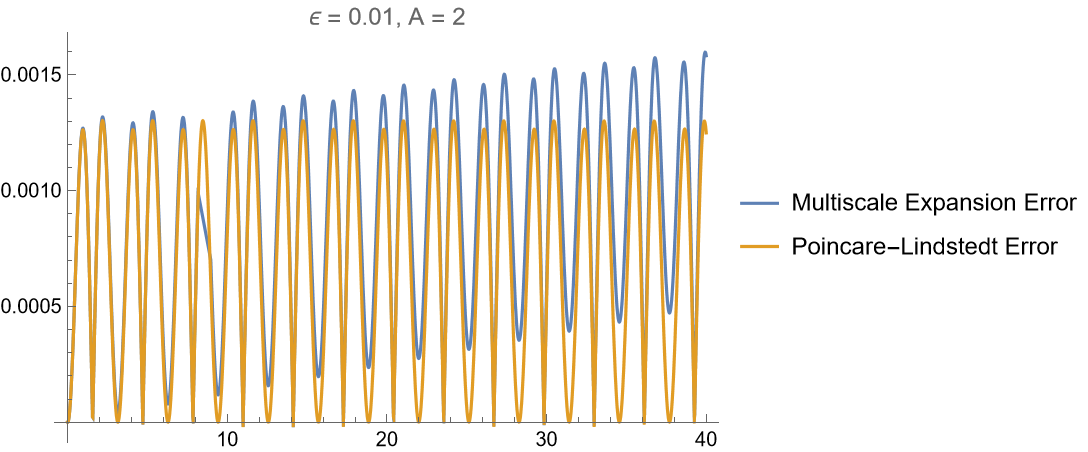
\includegraphics[width=.8\textwidth]{plots/2d1.png}
        \end{figure}
        \begin{figure}[H]
            \center
            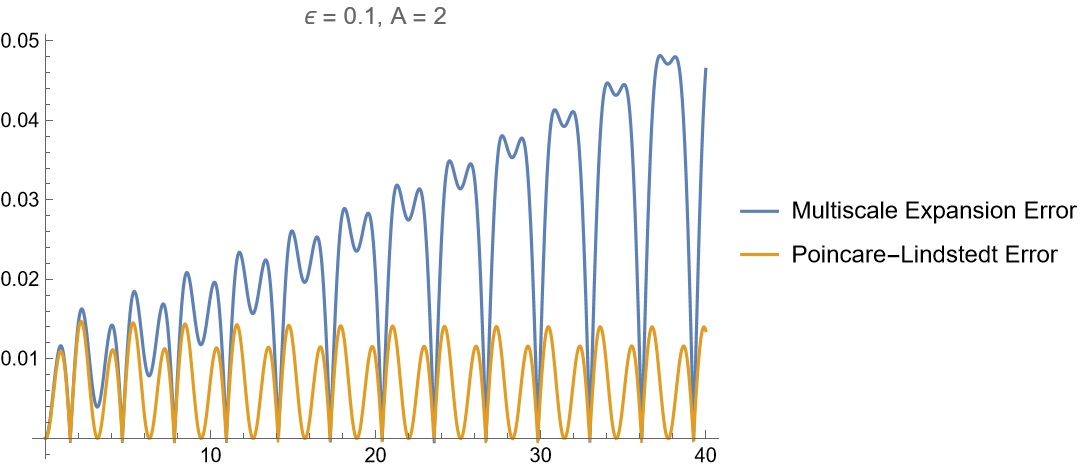
\includegraphics[width=.8\textwidth]{plots/2d2.png}
        \end{figure}
        \begin{figure}[H]
            \center
            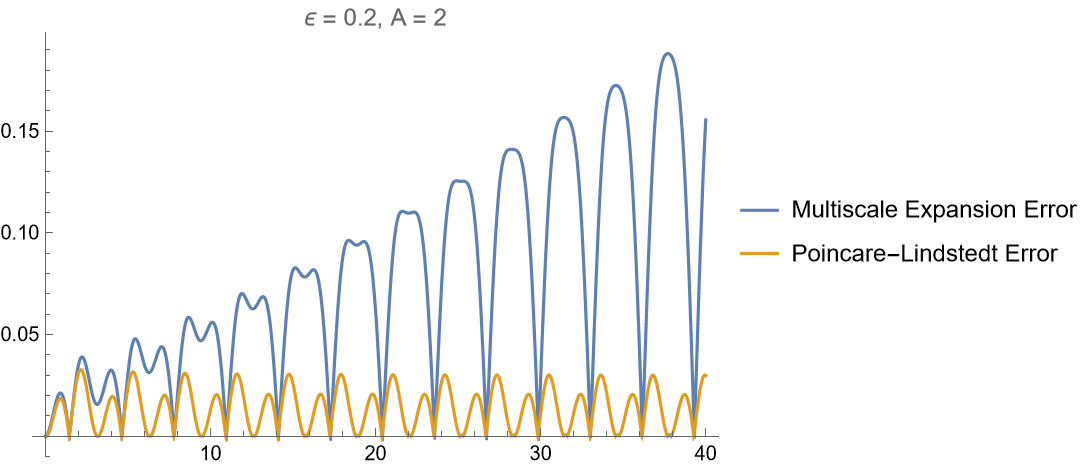
\includegraphics[width=.8\textwidth]{plots/2d3.png}
        \end{figure}
        \begin{figure}[H]
            \center
            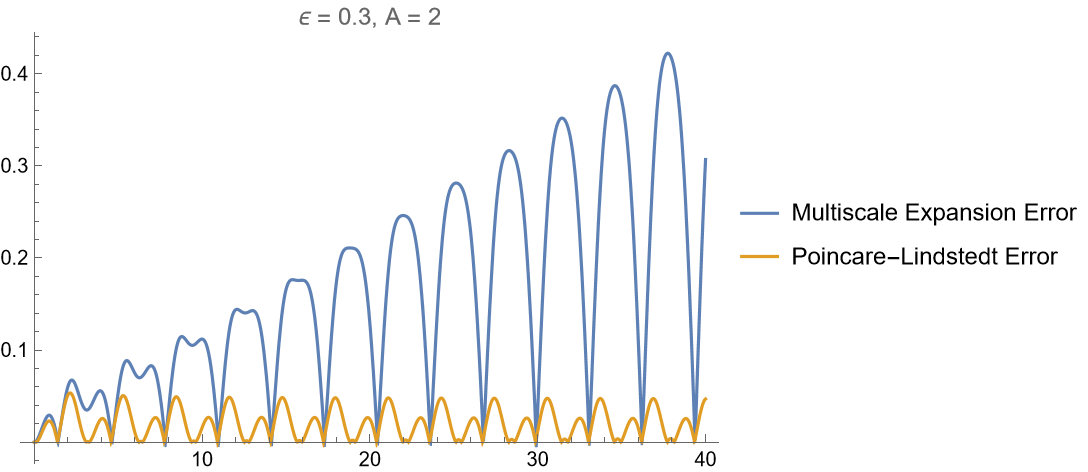
\includegraphics[width=.8\textwidth]{plots/2d4.png}
        \end{figure}
        
    \end{enumerate}
\end{solution}

%----------------------------------------------------------------------------------------------------%
%\vskip 20pt
\newpage

\end{document} 